\section{Visualisierung}
Auf Grund der hohen Dichte von möglichen Visualisierungselementen wird das Hochregallager aufgeklappt und vereinfacht dargestellt.
%
\subsection{Trennung}
Der Lagerwand und den involvierten Akteure wurde je eine Ebene (Layer) zugeweisen. Dies stellt sicher, dass bei der Darstellung nur die Elemente, welche sich seit dem letzten Schritt verändert haben, neu geladen werden müssten.  

%
\begin{figure}[h]
\subfigure[Lagergitter]{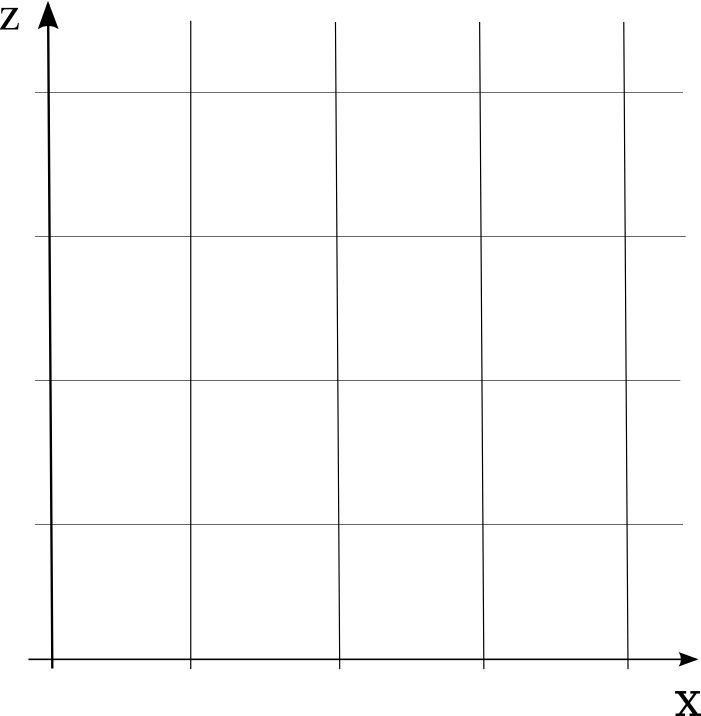
\includegraphics[width=0.29\textwidth]{images/lagergitter.png}}\hfill
\subfigure[Belegung]{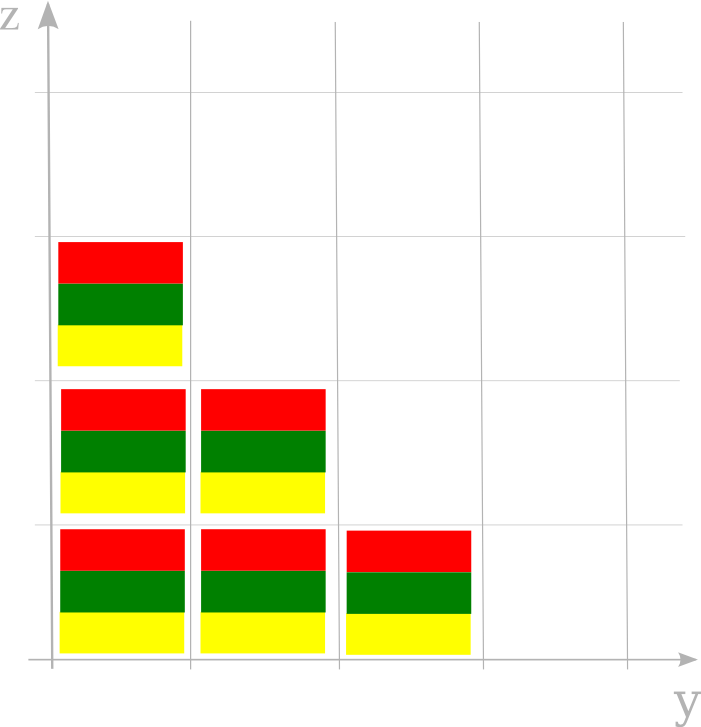
\includegraphics[width=0.29\textwidth]{images/belegung.png}}\hfill
\subfigure[Regalbediengerät]{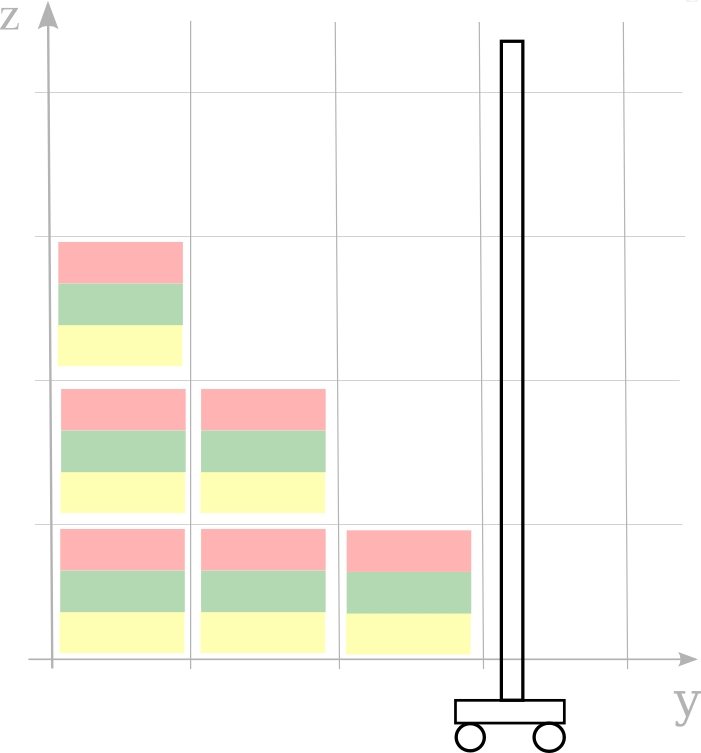
\includegraphics[width=0.29\textwidth]{images/rbg-arm.png}}
\caption{Trennungen}
\end{figure}

\begin{figure}[h]
\subfigure[Regalbediengerät-Ausleger]{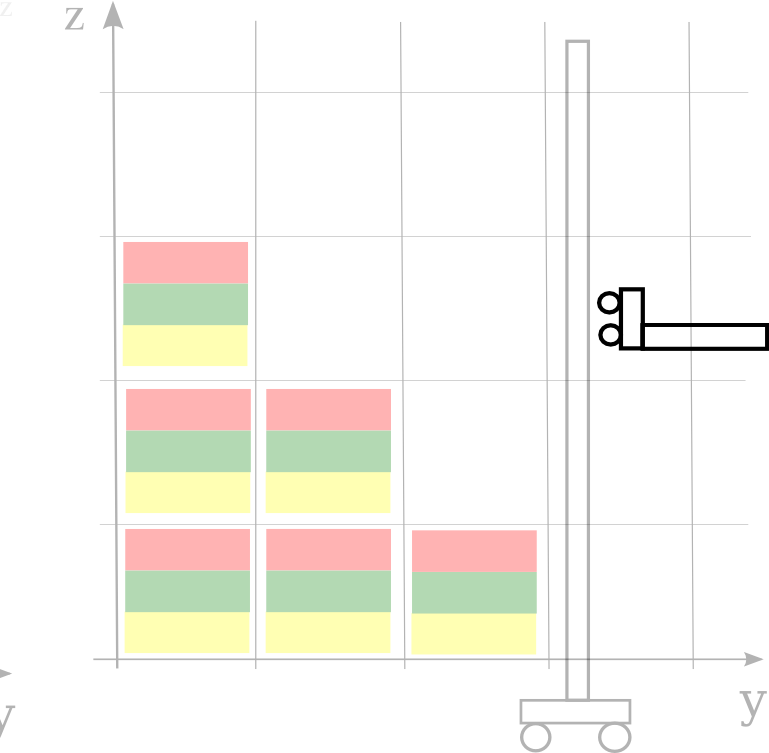
\includegraphics[width=0.29\textwidth]{images/rbg-ausleger.png}}\hfill
\subfigure[Lagergut]{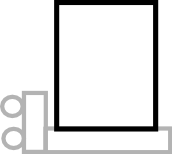
\includegraphics[width=0.19\textwidth]{images/lagergut.png}}
\caption{Weitere Trennungen}
\end{figure}
%

%EOF
